% Options for packages loaded elsewhere
\PassOptionsToPackage{unicode}{hyperref}
\PassOptionsToPackage{hyphens}{url}
\PassOptionsToPackage{dvipsnames,svgnames,x11names}{xcolor}
%
\documentclass[
]{estat/estat}

\usepackage{amsmath,amssymb}
\usepackage{iftex}
\ifPDFTeX
  \usepackage[T1]{fontenc}
  \usepackage[utf8]{inputenc}
  \usepackage{textcomp} % provide euro and other symbols
\else % if luatex or xetex
  \usepackage{unicode-math}
  \defaultfontfeatures{Scale=MatchLowercase}
  \defaultfontfeatures[\rmfamily]{Ligatures=TeX,Scale=1}
\fi
\usepackage{lmodern}
\ifPDFTeX\else  
    % xetex/luatex font selection
    \setmainfont[]{Arial}
\fi
% Use upquote if available, for straight quotes in verbatim environments
\IfFileExists{upquote.sty}{\usepackage{upquote}}{}
\IfFileExists{microtype.sty}{% use microtype if available
  \usepackage[]{microtype}
  \UseMicrotypeSet[protrusion]{basicmath} % disable protrusion for tt fonts
}{}
\makeatletter
\@ifundefined{KOMAClassName}{% if non-KOMA class
  \IfFileExists{parskip.sty}{%
    \usepackage{parskip}
  }{% else
    \setlength{\parindent}{0pt}
    \setlength{\parskip}{6pt plus 2pt minus 1pt}}
}{% if KOMA class
  \KOMAoptions{parskip=half}}
\makeatother
\usepackage{xcolor}
\usepackage[left=3cm,right=2cm,top=3cm,bottom=2cm]{geometry}
\setlength{\emergencystretch}{3em} % prevent overfull lines
\setcounter{secnumdepth}{5}
% Make \paragraph and \subparagraph free-standing
\makeatletter
\ifx\paragraph\undefined\else
  \let\oldparagraph\paragraph
  \renewcommand{\paragraph}{
    \@ifstar
      \xxxParagraphStar
      \xxxParagraphNoStar
  }
  \newcommand{\xxxParagraphStar}[1]{\oldparagraph*{#1}\mbox{}}
  \newcommand{\xxxParagraphNoStar}[1]{\oldparagraph{#1}\mbox{}}
\fi
\ifx\subparagraph\undefined\else
  \let\oldsubparagraph\subparagraph
  \renewcommand{\subparagraph}{
    \@ifstar
      \xxxSubParagraphStar
      \xxxSubParagraphNoStar
  }
  \newcommand{\xxxSubParagraphStar}[1]{\oldsubparagraph*{#1}\mbox{}}
  \newcommand{\xxxSubParagraphNoStar}[1]{\oldsubparagraph{#1}\mbox{}}
\fi
\makeatother


\providecommand{\tightlist}{%
  \setlength{\itemsep}{0pt}\setlength{\parskip}{0pt}}\usepackage{longtable,booktabs,array}
\usepackage{calc} % for calculating minipage widths
% Correct order of tables after \paragraph or \subparagraph
\usepackage{etoolbox}
\makeatletter
\patchcmd\longtable{\par}{\if@noskipsec\mbox{}\fi\par}{}{}
\makeatother
% Allow footnotes in longtable head/foot
\IfFileExists{footnotehyper.sty}{\usepackage{footnotehyper}}{\usepackage{footnote}}
\makesavenoteenv{longtable}
\usepackage{graphicx}
\makeatletter
\def\maxwidth{\ifdim\Gin@nat@width>\linewidth\linewidth\else\Gin@nat@width\fi}
\def\maxheight{\ifdim\Gin@nat@height>\textheight\textheight\else\Gin@nat@height\fi}
\makeatother
% Scale images if necessary, so that they will not overflow the page
% margins by default, and it is still possible to overwrite the defaults
% using explicit options in \includegraphics[width, height, ...]{}
\setkeys{Gin}{width=\maxwidth,height=\maxheight,keepaspectratio}
% Set default figure placement to htbp
\makeatletter
\def\fps@figure{htbp}
\makeatother

\authors{%
    Estatiano 1 \\
    Estatiano 2\\
    Estatiano 3\\
}

% escreva o nome do cliente aqui
% se for mais de um separe por \\
\client{%
    ESTAT
}
% Baixando pacotes
\RequirePackage{fancyhdr}
\RequirePackage{graphicx}

\setlength\headheight{28pt}  

\setlength{\parindent}{15pt} % Adiciona indentação nos parágrafos
\setlength{\parskip}{0pt} % Adiciona 0 espaço entro os parágrafos

\let\oldsection\section
\renewcommand\section{\clearpage\oldsection}
\makeatletter
\@ifpackageloaded{float}{}{\usepackage{float}}
\floatstyle{plain}
\@ifundefined{c@chapter}{\newfloat{quadro}{h}{loquad}}{\newfloat{quadro}{h}{loquad}[chapter]}
\floatname{quadro}{Quadro}
\floatstyle{plaintop}
\restylefloat{quadro}
\newcommand*\listofquadros{\listof{quadro}{List of Testes}}
\makeatother
\makeatletter
\@ifpackageloaded{caption}{}{\usepackage{caption}}
\AtBeginDocument{%
\ifdefined\contentsname
  \renewcommand*\contentsname{Índice}
\else
  \newcommand\contentsname{Índice}
\fi
\ifdefined\listfigurename
  \renewcommand*\listfigurename{Lista de Figuras}
\else
  \newcommand\listfigurename{Lista de Figuras}
\fi
\ifdefined\listtablename
  \renewcommand*\listtablename{Lista de Tabelas}
\else
  \newcommand\listtablename{Lista de Tabelas}
\fi
\ifdefined\figurename
  \renewcommand*\figurename{Figura}
\else
  \newcommand\figurename{Figura}
\fi
\ifdefined\tablename
  \renewcommand*\tablename{Tabela}
\else
  \newcommand\tablename{Tabela}
\fi
}
\@ifpackageloaded{float}{}{\usepackage{float}}
\floatstyle{ruled}
\@ifundefined{c@chapter}{\newfloat{codelisting}{h}{lop}}{\newfloat{codelisting}{h}{lop}[chapter]}
\floatname{codelisting}{Listagem}
\newcommand*\listoflistings{\listof{codelisting}{Lista de Listagens}}
\captionsetup{labelsep=colon}
\makeatother
\makeatletter
\makeatother
\makeatletter
\@ifpackageloaded{caption}{}{\usepackage{caption}}
\@ifpackageloaded{subcaption}{}{\usepackage{subcaption}}
\makeatother

\ifLuaTeX
\usepackage[bidi=basic]{babel}
\else
\usepackage[bidi=default]{babel}
\fi
\babelprovide[main,import]{portuguese}
\ifPDFTeX
\else
\babelfont{rm}[]{Arial}
\fi
% get rid of language-specific shorthands (see #6817):
\let\LanguageShortHands\languageshorthands
\def\languageshorthands#1{}
\ifLuaTeX
  \usepackage{selnolig}  % disable illegal ligatures
\fi
\usepackage{bookmark}

\IfFileExists{xurl.sty}{\usepackage{xurl}}{} % add URL line breaks if available
\urlstyle{same} % disable monospaced font for URLs
\hypersetup{
  pdflang={pt},
  colorlinks=true,
  linkcolor={black},
  filecolor={black},
  citecolor={black},
  urlcolor={black},
  pdfcreator={LaTeX via pandoc}}


\author{}
\date{}

\begin{document}

% Limpando tudo
\fancyhf{} 

% Ajustes do header
\fancyhead[L]{} % limpando o lado esquerdo
\fancyhead[R]{\includegraphics[width=0.20\textwidth]{estat/imagens/estat.png}} % adicionando logo no canto direito
\renewcommand{\headrulewidth}{0pt}   % sem linha embaixo da logo

% Ajustes de fim de página
\fancyfoot[R]{\textcolor{white}{\thepage}} % Número em branco no canto direito

% Aplicando o estilo que acabamos de criar
\pagestyle{fancy} 


\labelformat{quadro}{\textbf{#1}}

\renewcommand*\contentsname{Sumário}
{
\hypersetup{linkcolor=}
\setcounter{tocdepth}{3}
\tableofcontents
}

\section{Introdução}\label{introduuxe7uxe3o}

O seguinte projeto tem por objetivo apresentar as análises estatísticas
requisitadas pelo Diretor Financeiro da Phineas \& Ferb Capital, Felipe
Bretas, buscando compreender os principais fatores que influenciam a
inflação para a oferta de subsídios para a formulação de políticas
econômicas mais assertivas, por meio de análises detalhadas que
evidenciam tendências, variações e correlações ao longo dos anos de 2002
a 2022.

Para cumprir esse objetivo, foi solicitado estudos sobre o impacto da
Taxa Selic na inflação e nos juros reais, a relação sobre a Taxa Selic e
a inflação e a distribuição do salario mínimo ao longo dos mandatos
presidenciais. Para a realização dessas análises, foi utilizado gráficos
de dispersão, linhas e boxplot, além de coeficientes de correlação. Para
a realização do projeto foi utilizado o banco de dados inflacao em
formato csv, disponibilizado pelo próprio cliente. Para a produção do
relatório foram abordadas apenas algumas variáveis presentes no banco de
dados, essas sendo a Taxa Selic, a taxa básica de juros da economia
brasileira, o IPCA acumulado, que indica a inflação no país, o salario
minimo, que indica o menor salario que um individuo pode receber e o ano
de cada informação.

O software utilizado para análise estatística dos dados foi o R versão
4.4.2.. O R é um software de programação gratuito largamente usado na
área de estatística e visualização de dados que permite não só o
manuseio e análise de bancos de dados, como também a confecção de
gráficos.

\section{Referencial Teórico}\label{referencial-teuxf3rico}

\subsection{Frequência Relativa}\label{frequuxeancia-relativa}

A frequência relativa é utilizada para a comparação entre classes de uma
variável categórica com \(c\) categorias, ou para comparar uma mesma
categoria em diferentes estudos.

A frequência relativa da categoria \(j\) é dada por:

\[
f_j=\frac{n_j}{n}
\]

Com:

\begin{itemize}
\item
  \(j = 1, \, ..., \, c\)
\item
  \(n_j =\) número de observações da categoria \(j\)
\item
  \(n =\) número total de observações
\end{itemize}

Geralmente, a frequência relativa é utilizada em porcentagem, dada por:

\[100 \times f_j\]

\subsection{Média}\label{muxe9dia}

A média é a soma das observações dividida pelo número total delas, dada
pela fórmula:

\[\bar{X}=\frac{\sum\limits_{i=1}^{n}X_i}{n}\]

Com:

\begin{itemize}
\item
  \(i = 1, \, 2, \, ..., \, n\)
\item
  \(n =\) número total de observações
\end{itemize}

\subsection{Mediana}\label{mediana}

Sejam as \(n\) observações de um conjunto de dados
\(X=X_{(1)},X_{(2)},\ldots, X_{(n)}\) de determinada variável ordenadas
de forma crescente. A mediana do conjunto de dados \(X\) é o valor que
deixa metade das observações abaixo dela e metade dos dados acima.

Com isso, pode-se calcular a mediana da seguinte forma:

\[
med(X) =
    \begin{cases}
         X_{\frac{n+1}{2}}, \textrm{para n ímpar} \\
         \frac{X_{\frac{n}{2}}+X_{\frac{n}{2} + 1}}{2}, \textrm{para n par} \\
    \end{cases}
\]

\subsection{Quartis}\label{quartis}

Os quartis são separatrizes que dividem o conjunto de dados em quatro
partes iguais. O primeiro quartil (ou inferior) delimita os 25\% menores
valores, o segundo representa a mediana, e o terceiro delimita os 25\%
maiores valores. Inicialmente deve-se calcular a posição do quartil:

\begin{itemize}
\item
  Posição do primeiro quartil \(P_1\): \[P_1=\frac{n+1}{4}\]
\item
  Posição da mediana (segundo quartil) \(P_2\): \[P_2 = \frac{n+1}{2}\]
\item
  Posição do terceiro quartil \(P_3\): \[P_3=\frac{3 \times (n+1)}{4}\]
\end{itemize}

Com \(n\) sendo o tamanho da amostra. Dessa forma,
\(X_{\left( P_i \right)}\) é o valor do \(i\)-ésimo quartil, onde
\(X_{\left( j \right)}\) representa a \(j\)-ésima observação dos dados
ordenados.

Se o cálculo da posição resultar em uma fração, deve-se fazer a média
entre o valor que está na posição do inteiro anterior e do seguinte ao
da posição.

\subsection{Variância}\label{variuxe2ncia}

A variância é uma medida que avalia o quanto os dados estão dispersos em
relação à média, em uma escala ao quadrado da escala dos dados.

\subsubsection{Variância Populacional}\label{variuxe2ncia-populacional}

Para uma população, a variância é dada por:

\[\sigma^2=\frac{\sum\limits_{i=1}^{N}\left(X_i - \mu\right)^2}{N}\]

Com:

\begin{itemize}
\item
  \(X_i =\) \(i\)-ésima observação da população
\item
  \(\mu =\) média populacional
\item
  \(N =\) tamanho da população
\end{itemize}

\subsection{Desvio Padrão}\label{desvio-padruxe3o}

O desvio padrão é a raiz quadrada da variância. Ele avalia o quanto os
dados estão dispersos em relação à média.

\subsubsection{Desvio Padrão
Populacional}\label{desvio-padruxe3o-populacional}

Para uma população, o desvio padrão é dado por:

\[\sigma=\sqrt{\frac{\sum\limits_{i=1}^{N}\left(X_i - \mu\right)^2}{N}}\]

Com:

\begin{itemize}
\item
  \(X_i =\) i-ésima observação da população
\item
  \(\mu =\) média populacional
\item
  \(N =\) tamanho da população
\end{itemize}

\subsection{Boxplot}\label{boxplot}

O boxplot é uma representação gráfica na qual se pode perceber de forma
mais clara como os dados estão distribuídos. A figura abaixo ilustra um
exemplo de boxplot.

\begin{figure}[H]

\caption{Exemplo de boxplot}

{\centering \includegraphics{images/box_uni.png}

}

\end{figure}%

A porção inferior do retângulo diz respeito ao primeiro quartil,
enquanto a superior indica o terceiro quartil. Já o traço no interior do
retângulo representa a mediana do conjunto de dados, ou seja, o valor em
que o conjunto de dados é dividido em dois subconjuntos de mesmo
tamanho. A média é representada pelo losango branco e os pontos são
\emph{outliers}. Os \emph{outliers} são valores discrepantes da série de
dados, ou seja, valores que não demonstram a realidade de um conjunto de
dados.

\subsection{Gráfico de Dispersão}\label{gruxe1fico-de-dispersuxe3o}

O gráfico de dispersão é uma representação gráfica utilizada para
ilustrar o comportamento conjunto de duas variáveis quantitativas. A
figura abaixo ilustra um exemplo de gráfico de dispersão, onde cada
ponto representa uma observação do banco de dados.

\begin{figure}[H]

\caption{Exemplo de Gráfico de Dispersão}

{\centering 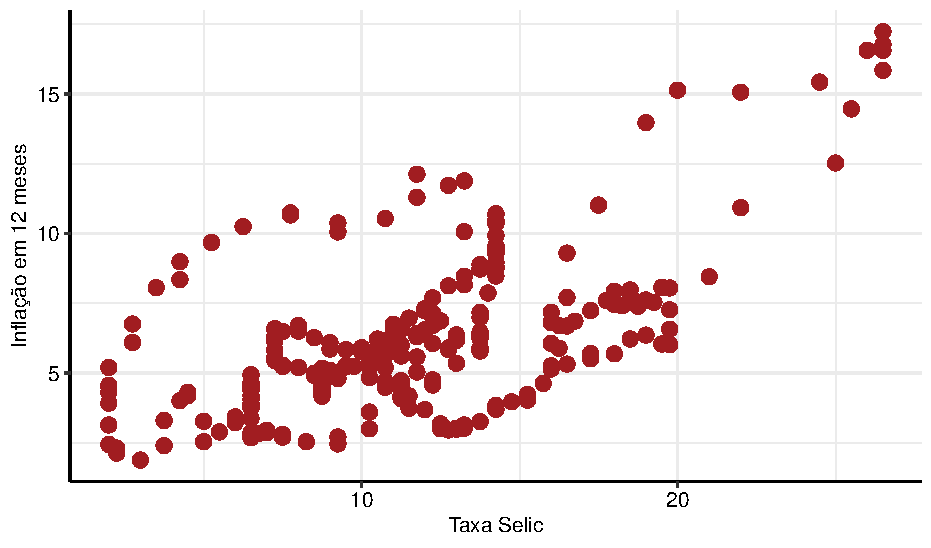
\includegraphics{images/disp_uni.png}

}

\end{figure}%

\subsection{Tipos de Variáveis}\label{tipos-de-variuxe1veis}

\subsubsection{Qualitativas}\label{qualitativas}

As variáveis qualitativas são as variáveis não numéricas, que
representam categorias ou características da população. Estas
subdividem-se em:

\begin{itemize}
\tightlist
\item
  \textbf{Nominais}: quando não existe uma ordem entre as categorias da
  variável (exemplos: sexo, cor dos olhos, fumante ou não, etc)
\item
  \textbf{Ordinais}: quando existe uma ordem entre as categorias da
  variável (exemplos: nível de escolaridade, mês, estágio de doença,
  etc)
\end{itemize}

\subsubsection{Quantitativas}\label{quantitativas}

As variáveis quantitativas são as variáveis numéricas, que representam
características numéricas da população, ou seja, quantidades. Estas
subdividem-se em:

\begin{itemize}
\tightlist
\item
  \textbf{Discretas}: quando os possíveis valores são enumeráveis
  (exemplos: número de filhos, número de cigarros fumados, etc)
\item
  \textbf{Contínuas}: quando os possíveis valores são resultado de
  medições (exemplos: massa, altura, tempo, etc)
\end{itemize}

\subsection{Coeficiente de Correlação de
Pearson}\label{coeficiente-de-correlauxe7uxe3o-de-pearson}

O coeficiente de correlação de Pearson é uma medida que verifica o grau
de relação linear entre duas variáveis quantitativas. Este coeficiente
varia entre os valores -1 e 1. O valor zero significa que não há relação
linear entre as variáveis. Quando o valor do coeficiente \(r\) é
negativo, diz-se existir uma relação de grandeza inversamente
proporcional entre as variáveis. Analogamente, quando \(r\) é positivo,
diz-se que as duas variáveis são diretamente proporcionais.

O coeficiente de correlação de Pearson é normalmente representado pela
letra \(r\) e a sua fórmula de cálculo é:

\[
r_{Pearson} = \frac{\displaystyle \sum_{i=1}^{n} \left [ \left(x_i-\bar{x}\right) \left(y_i-\bar{y}\right) \right]}{\sqrt{\displaystyle \sum_{i=1}^{n} x_i^2 - n\bar{x}^2}  \times \sqrt{\displaystyle \sum_{i=1}^{n} y_i^2 - n\bar{y}^2}}
\]

Onde:

\begin{itemize}
\tightlist
\item
  \(x_i =\) i-ésimo valor da variável \(X\)
\item
  \(y_i =\) i-ésimo valor da variável \(Y\)
\item
  \(\bar{x} =\) média dos valores da variável \(X\)
\item
  \(\bar{y} =\) média dos valores da variável \(Y\)
\end{itemize}

Vale ressaltar que o coeficiente de Pearson é paramétrico e, portanto,
sensível quanto à normalidade (simetria) dos dados.

\section{Análises}\label{anuxe1lises}

\subsection{Relação entre Taxa Selic, Inflação Acumulada e Juros ao
longo do
tempo}\label{relauxe7uxe3o-entre-taxa-selic-inflauxe7uxe3o-acumulada-e-juros-ao-longo-do-tempo}

Na primeira análise, foi examinada a relação entre a variável
quantitativa contínua Taxa Selic, que representa a taxa básica de juros,
e as variáveis quantitativas contínuas Inflação Acumulada e Juros Reais,
no período de 2002 a 2022. Para representar esses dados, foi feita uma
média dessas variáveis em cada ano para a utilização de um gráfico de
linhas multivariado, gráfico esse que é utilizado para análises
temporais.

\begin{figure}[H]

\caption{\label{fig-graf1}Gráfico de linha do IPCA acumulado em doze
meses, juros reais e Taxa Selic ao longo do tempo}

\centering{

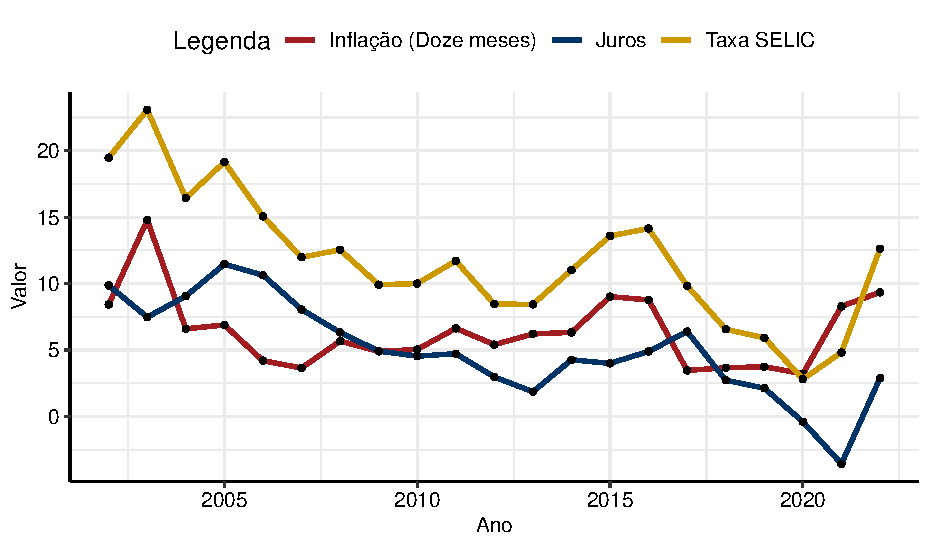
\includegraphics{antonio_files/figure-pdf/fig-graf1-1.pdf}

}

\end{figure}%

Ao observar a \(\ref{fig-graf1}\), é possivel notar que, no geral,
quando a Taxa Selic sofria uma alteração, a Inflação Acumulada e os
Juros sofriam uma alteração similiar. Pode-se perceber também que nos
anos de 2005, 2006 e 2021, as váriaveis apresentaram comportamentos
similiares, embora o comportamento nos demais anos tenha demonstrado uma
relação entre a inflação e a Taxa Selic. É interessante notar também que
ao comparar os valores nos anos de 2002 e 2022, apenas a inflação
apresenta um crescimento em comparação com seu valor de 20 anos
anteriores, contrastando com a taxa Selic que apresentou a maior redução
entre as três.

\subsection{Estudo da correlação entre Inflação Acumulada e a Taxa
Selic}\label{estudo-da-correlauxe7uxe3o-entre-inflauxe7uxe3o-acumulada-e-a-taxa-selic}

O presente estudo tem como objeto de análise a relação entre as
variáveis quantitativas contínuas: inflação acumulada, representada pelo
IPCA acumulado em doze meses, e a Taxa Selic. O objetivo desta
investigação é compreender o impacto da inflação sobre a Taxa Selic, que
constitui a taxa básica de juros da economia. Para isso, foram
utilizados o gráfico de dispersão bivariado e o Coeficiente de
Correlação de Pearson, proporcionando uma melhor compreensão das
interações entre as variáveis analisadas.

\begin{figure}[H]

\caption{\label{fig-graf2}Gráfico de dispersão de Inflação Acumulada
pela Taxa Selic}

\centering{

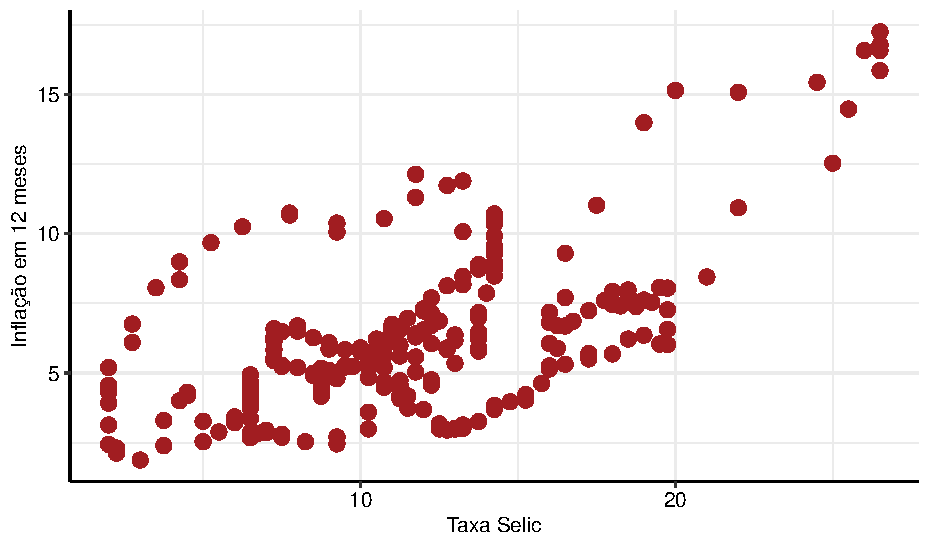
\includegraphics{antonio_files/figure-pdf/fig-graf2-1.pdf}

}

\end{figure}%

Pode ser observado na \(\ref{fig-graf2}\) que existe uma correlação
entre as variáveis, o que pode ser comprovado pelo Coeficiente de
Correlação de Pearson, utilizado para indentificar a relação linear de
variáveis quantitativas, que assume o valor aproximado de 0.635,
significando uma relação média a forte entre as váriaveis Inflação
Acumulada e a Taxa Selic. Isso indica uma tendência da inflação sofrer
alterações similiares a Taxa Selic.

\subsection{Variação de salario mínimo por mandato
presidencial}\label{variauxe7uxe3o-de-salario-muxednimo-por-mandato-presidencial}

Nesta análise, será observada a evolução da variável quantitativa
contínua `salário mínimo' durante o mandato de cada presidente. A
variável qualitativa nominal corresponde aos diferentes presidentes no
período de 2002 a 2022, incluindo: o final do mandato de Fernando
Henrique Cardoso em 2002, abreviado para FHC; os dois mandatos de Luiz
Inácio Lula da Silva e Dilma Rousseff, abreviados como `Lula' e `Dilma',
respectivamente, seguidos pelo número do mandato; Michael Temer,
abreviado como `Temer', que assumiu a maior parte do mandato seguinte ao
segundo de Dilma; e Jair Bolsonaro, apresentado como `Bolsonaro' no
gráfico. As eleições ocorrem a cada quatro anos, sendo o ano eleitoral
considerado como o último ano de cada mandato. Isso fez com que as
informações referentes a 2002 fossem menos precisas. Para realizar essa
análise, foi utilizado um gráfico de boxplot.

\begin{figure}[H]

\caption{\label{fig-graf3}Gráfico boxplot do Salario mínimo por mandato}

\centering{

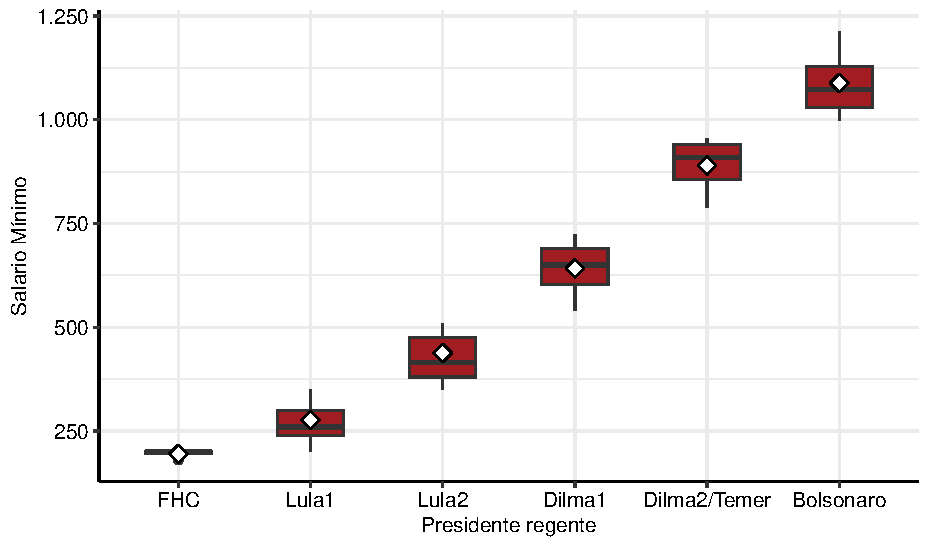
\includegraphics{antonio_files/figure-pdf/fig-graf3-1.pdf}

}

\end{figure}%

\begin{quadro}[H]

\caption{\label{quad-sal-min}Quadro de medidas resumo do salário mínimo
por mandato presidencial}

\centering{

\begin{tabular}{|l|l|l|l|l|l|l|}
\hline
\textbf{Medidas Resumo} & \textbf{FHC} & \textbf{Lula1} & \textbf{Lula2} & \textbf{Dilma1} & \textbf{Dilma2/Temer} & \textbf{Bolsonaro} \\ \hline
Média                   & 195          & 276,88         & 438,12         & 642,04         & 889,75                & 1088,62           \\
Desvio Padrão           & 9,04        & 44,44          & 53,85          & 67,78          & 65,51                & 80,70             \\
Variância               & 81,90       & 1974,91        & 2899,82        & 4594,39        & 4291,56              & 6513,94           \\
1° Quartil              & 195          & 240            & 380            & 602,75          & 857                   & 1028,75            \\
Mínimo                  & 180          & 200            & 350            & 540             & 788                   & 998                \\
Mediana                 & 200          & 260            & 415            & 650             & 908,5                 & 1072,5             \\
Máximo                  & 200          & 350            & 510            & 724             & 954                   & 1212               \\
3° Quartil              & 200          & 300            & 476,25         & 689,5           & 941,25                & 1128               \\ \hline
\end{tabular}

}

\end{quadro}%

Como pode ser percebido pela \(\ref{fig-graf3}\), assim como no
\textbf{Quadro}~\ref{quad-sal-min}, o salário mínimo aumentou com o
tempo. Isso pode ser notado observando como as medianas na
\(\ref{fig-graf3}\) sobem a cada mandato, o que também pode ser visto no
\textbf{Quadro}~\ref{quad-sal-min}. Nota-se também o aumento do desvio
padrão, medida utilizada para entender a dispersão dos valores.

O mandato com a maior variação entre o menor e o maior salário foi o de
Jair Bolsonaro, com 214 reais de diferença, enquanto o menor, com
exceção do mandato de Fernando Henrique Cardoso que tem uma variação de
apenas 20 reais por apresentar apenas um ano, foi o primeiro mandato de
Lula, com 150 reais de diferença. Além disso, o maior aumento da média
salarial entre mandatos ocorreu nas duas posses de Dilma, com um aumento
de 203,92 reais, e o menor, novamente com a exceção do mandato de FHC
com uma diferença de 81,88, foi entre os mandatos de Lula, de 161,24.

Pode-se perceber então que não existem evidências de um aumento muito
grande do salário dentro do mandato e de um para o outro, flutuando por
volta de 150 e 200 reais em ambos os casos, em comparação entre os
analisados.

\section{Conclusão}\label{conclusuxe3o}

Após a realização de todas as análises, o objetivo da pesquisa, a
compreensão dos fatores que ifluenciam a inflação, pôde ser bem
explorado pelas análises.

Primeiramente na análise da relação entre inflação, Taxa Selic e Juros
Reais, foi possível perceber que por mais que eles influenciem um no
outro, ainda existem mais fatores não estudados nessa análise que afetam
essas variáveis.

Assim como na primeira análise apresentada, no estudo entre a relação da
Taxa Selic e da inflação acumulada em 12 meses, embora haja uma relação
média-forte entre as duas, ainda existem fatores não estudados que
influenciam essas variáveis.

Por fim, ao observar a variação do salário em cada mandato presidencial,
pode se perceber que a alteração de salário em cada mandato, assim como
de um mandato para outro não foi muito elevada ao fazer uma comparação
entre eles.




\end{document}
